\hypertarget{hypothesis-testing}{%
\chapter{Hypothesis Testing}\label{hypothesis-testing}}

This chapter introduces statistical hypothesis testing, which is such a
contentious topic in the history of statistics, it's hard to provide a
simple definition. Instead, I'll start with an example, present the
problem hypothesis testing is intended to solve, and then show a
solution.

The solution I'll show is different from what you might find in a
statistics book. Instead of mathematical analysis, we will use
computational simulations. This approach has two advantages and one
disadvantage:

\begin{itemize}
\item
  Advantage: The standard statistics curriculum includes many different
  tests, and many people find it hard to remember which one to use. In
  my opinion, simulation makes it clearer that there is only one testing
  framework.
\item
  Advantage: Simulations make modeling decision explicit. All
  statistical methods are based on models, but when we use mathematical
  methods, it is easy to forget the assumptions they are based on. With
  computation, the assumptions are more visible, and it is easier to try
  different models.
\item
  Disadvantage: Simulation uses a lot of computation. Some of the
  examples in this notebook take several seconds to run; for some of
  them, there are analytic methods that are much faster.
\end{itemize}

The examples in this chapter include results from a clinical trial
related to peanut allergies, and survey data from the National Survey of
Family Growth (NSFG) and the Behavioral Risk Factor Surveillance System
(BRFSS).

\hypertarget{testing-medical-treatments}{%
\section{Testing Medical Treatments}\label{testing-medical-treatments}}

The LEAP study was a randomized trial that tested the effect of eating
peanut snacks on the development of peanut allergies (see
\url{http://www.leapstudy.co.uk/leap-0\#.YEJax3VKikA}). The subjects
were infants who were at high risk of developing peanut allergies
because they had been diagnosed with other food allergies. Over a period
of several years, half of the subjects were periodically given a snack
containing peanuts; the other half were given no peanuts at all.

The conclusion of the study, reported in 2015 is:

\begin{quote}
Of the children who avoided peanut, 17\% developed peanut allergy by the
age of 5 years. Remarkably, only 3\% of the children who were randomized
to eating the peanut snack developed allergy by age 5. Therefore, in
high-risk infants, sustained consumption of peanut beginning in the
first 11 months of life was highly effective in preventing the
development of peanut allergy.
\end{quote}

These results seem impressive, but as skeptical data scientists we
should wonder whether it is possible that we are getting fooled by
randomness. Maybe the apparent difference between the groups is due to
chance, not the effectiveness of the treatment. To see whether this is
likely, we will simulate the experiment using a model where the
treatment has no effect, and see how often we see such a big difference
between the groups.

Detailed results of the study are reported in the \emph{New England
Journal of Medicine} (see
\url{https://www.nejm.org/doi/full/10.1056/NEJMoa1414850}). In that
article, Figure 1 shows the number of subjects in the treatment and
control groups, which happened to be equal.

\begin{lstlisting}[]
n_control = 314
n_treatment = 314
\end{lstlisting}

And from Figure 2 we can extract the number of subjects who developed
peanut allergies in each group. Specifically, we'll use the numbers from
the ``intention to treat analysis for both cohorts''.

\begin{lstlisting}[]
k_control = 54
k_treatment = 10
\end{lstlisting}

Using these numbers, we can compute the risk in each group as a
percentage.

\begin{lstlisting}[]
risk_control = k_control / n_control * 100
risk_control
(@\dashfill@)
@@@17.197452229299362@@@
\end{lstlisting}

\begin{lstlisting}[]
risk_treatment = k_treatment / n_treatment * 100
risk_treatment
(@\dashfill@)
@@@3.1847133757961785@@@
\end{lstlisting}

These are consistent with the percentages reported in the paper. To
quantify the difference between the groups, we'll use relative risk,
which is the ratio of the risks in the two groups.

\begin{lstlisting}[]
relative_risk_actual = risk_treatment / risk_control
relative_risk_actual
(@\dashfill@)
@@@0.1851851851851852@@@
\end{lstlisting}

The risk in the treatment group is about 18\% of the risk in the control
group. So it seems like the treatment is highly effective. To check,
let's imagine a world where the treatment is completely ineffective, so
the risk is actually the same in both groups, and the difference we saw
is due to chance. If that's true, we can estimate the hypothetical risk
by combining the two groups:

\begin{lstlisting}[]
n_all = n_control + n_treatment
k_all = k_control + k_treatment
risk_all = k_all / n_all
risk_all
(@\dashfill@)
@@@0.10191082802547771@@@
\end{lstlisting}

If the risk is the same for both groups, it is close to 10\%. Now we can
use this hypothetical risk to simulate the experiment. Here's
\passthrough{\lstinline!simulate\_group\_percent!}, which we saw in
Chapter 11. It takes as parameters the size of the group,
\passthrough{\lstinline!n!}, and the risk, \passthrough{\lstinline!p!}.
It simulates the experiment and returns the number of cases as a
percentage of the group, which is the observed risk.

\begin{lstlisting}[]
import numpy as np

def simulate_group_percent(n, p):
    xs = np.random.random(size=n)
    k = np.sum(xs < p)
    return k / n * 100
\end{lstlisting}

If we call this function many times, the result is a list of observed
risks, one for each simulated experiment. Here's the list for the
treatment group.

\begin{lstlisting}[]
t1 = [simulate_group_percent(n_treatment, risk_all)
      for i in range(1000)]
\end{lstlisting}

And the control group.

\begin{lstlisting}[]
t2 = [simulate_group_percent(n_control, risk_all)
      for i in range(1000)]
\end{lstlisting}

If we divide these lists elementwise, the result is a list of relative
risks, one for each simulated experiment.

\begin{lstlisting}[]
relative_risks = np.divide(t2, t1)
\end{lstlisting}

We can use a KDE plot to visualize the distribution of these results.

\begin{lstlisting}[]
import matplotlib.pyplot as plt
import seaborn as sns

sns.kdeplot(relative_risks)

plt.xlabel('Relative risk')
plt.ylabel('Probability density')
plt.title('Relative risks from simulation with risk_all');
\end{lstlisting}

\begin{center}
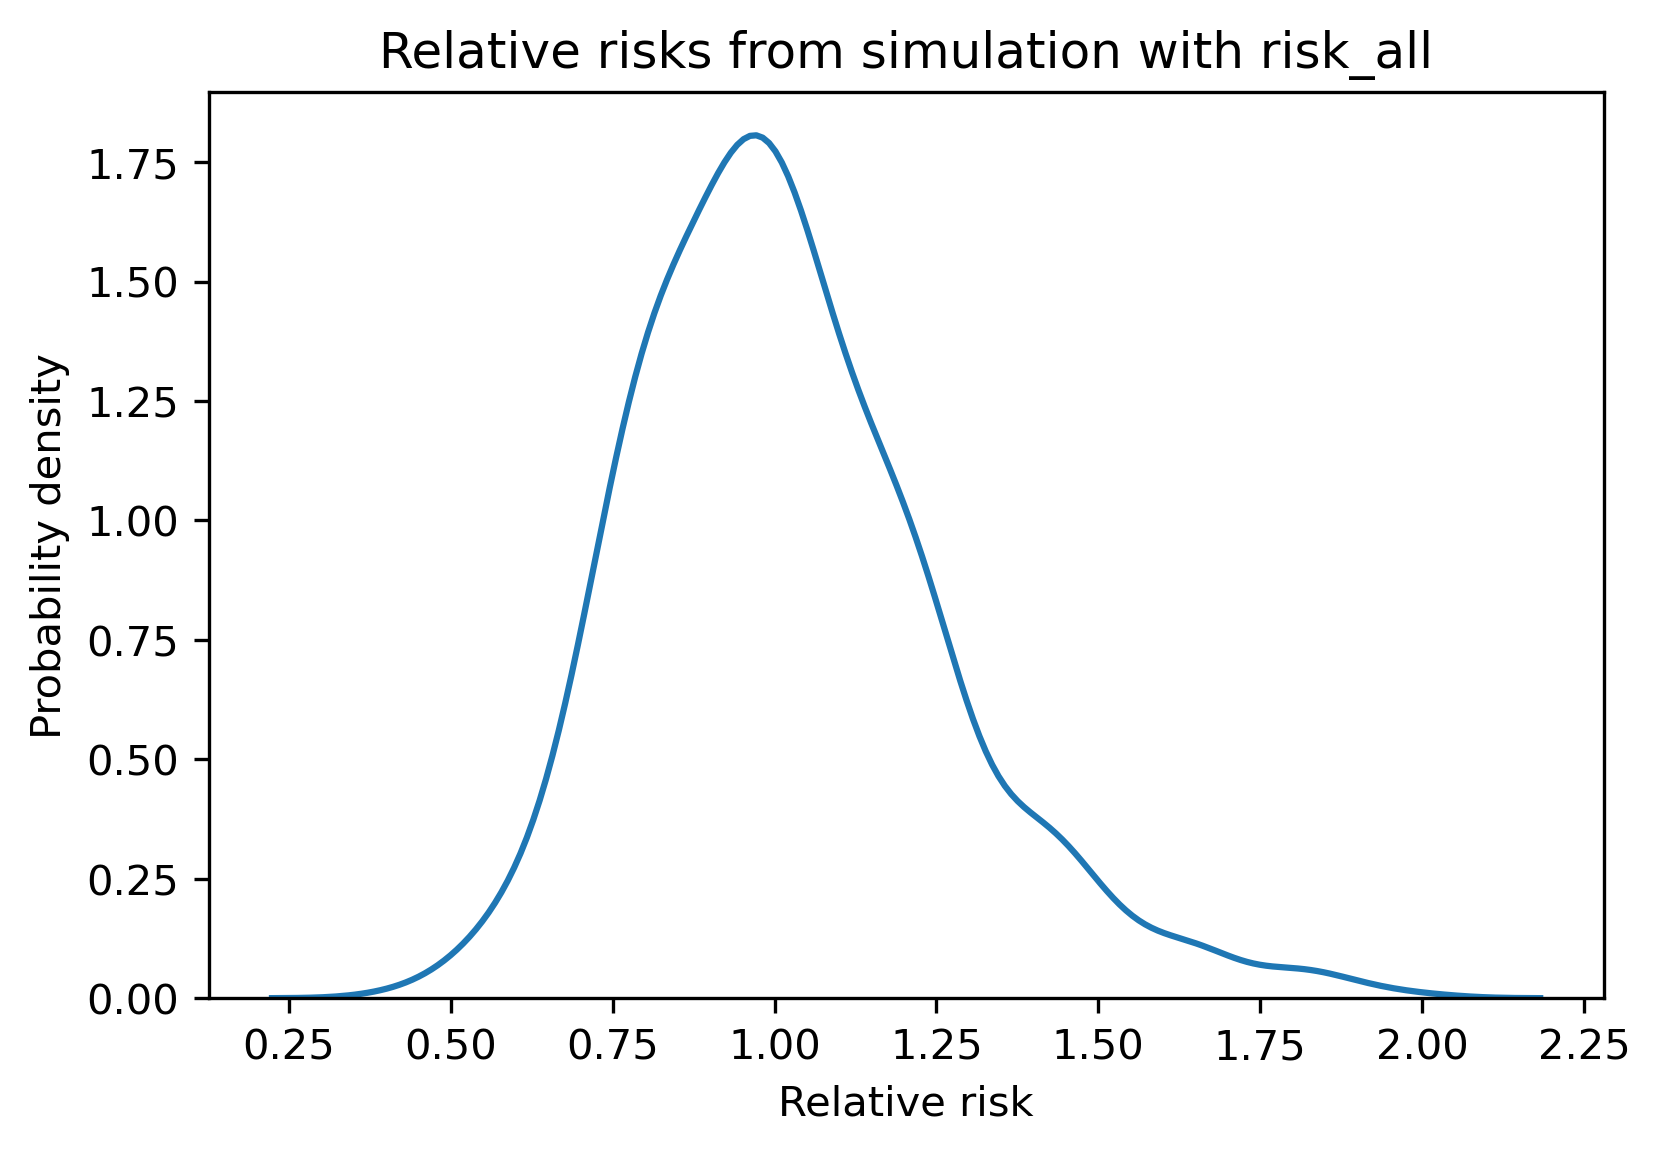
\includegraphics[width=4in]{chapters/13_hypothesis_files/13_hypothesis_27_0.png}
\end{center}

Remember that these simulations are based on the assumption that the
risk is the same for both groups, so we expect the relative risk to be
near 1 most of the time. And it is.

In some simulated experiments, the relative risk is as low as 0.5 or as
high as 2, which means it is plausible we could see results like that by
chance, even if there is no difference between groups.

But the relative risk in the actual experiment was 0.18, and we never
see a result as small as that in the simulated experiment. We can
conclude that the relative risk we saw is unlikely if the risk is
actually the same in both groups.

\hypertarget{computing-p-values}{%
\section{Computing p-values}\label{computing-p-values}}

Now suppose that in addition to the treatment and control groups, the
experiment included a placebo group that was given a snack that
contained no peanuts. Suppose this group was the same size as the
others, and 42 of the subjects developed peanut allergies.

To be clear, there was no third group, and I made up these numbers, but
let's see how this hypothetical works out. Here's the risk in the
placebo group.

\begin{lstlisting}[]
n_placebo = 314
k_placebo = 42

risk_placebo = k_placebo / n_placebo * 100
risk_placebo
(@\dashfill@)
@@@13.375796178343949@@@
\end{lstlisting}

And here's the relative risk compared to the control group.

\begin{lstlisting}[]
relative_risk_placebo = risk_placebo / risk_control
relative_risk_placebo
(@\dashfill@)
@@@0.7777777777777778@@@
\end{lstlisting}

The relative risk is less than 1, which means the risk in the placebo
group is a bit lower than in the control group. So we might wonder
whether the placebo was actually effective. To answer that question, at
least partially, we can go back to the results from the simulated
experiment.

Under the assumption that there is actually no difference between the
groups, it would not be unusual to see a relative risk as low as 0.77 by
chance. In fact, we can compute the probability of seeing a relative
risk as low or lower than
\passthrough{\lstinline!relative\_risk\_placebo!}, even if the two
groups are the same, like this:

\begin{lstlisting}[]
p_value = (relative_risks <= relative_risk_placebo).mean()
p_value
(@\dashfill@)
@@@0.137@@@
\end{lstlisting}

This probability is called a \textbf{p-value} (see
\url{https://en.wikipedia.org/wiki/P-value}). In this case, the p-value
is about 14\%, which means that even if the two groups are the same, we
expect to see a relative risk as low as 0.77 about 14\% of the time. So,
for this imagined experiment, we can't rule out the possibility that the
apparent difference is due to chance.

\hypertarget{are-first-babies-more-likely-to-be-late}{%
\section{Are First Babies More Likely To Be
Late?}\label{are-first-babies-more-likely-to-be-late}}

In the previous example, we saw a difference in proportion between two
groups. As a second example, let's consider a difference in means.

When my wife and I were expecting our first child, we heard that first
babies are more likely to be born late. But we also heard that first
babies are more likely to be born early. So which is it? As a data
scientist with too much time on my hands, I decided to find out. I got
data from the National Survey of Family Growth (NSFG), the same survey
we have used in previous chapters. I've put the results from the
2015-2017 survey in an HDF file. Here are the first few rows.

\begin{lstlisting}[]
import pandas as pd

nsfg = pd.read_hdf('nsfg.hdf', 'nsfg')
nsfg.head()
(@\dashfill@)
@@@/home/downey/miniconda3/envs/ElementsOfDataScience/lib/python3.8/site-packages/IPython/core/formatters.py:342: FutureWarning: In future versions `DataFrame.to_latex` is expected to utilise the base implementation of `Styler.to_latex` for formatting and rendering. The arguments signature may therefore change. It is recommended instead to use `DataFrame.style.to_latex` which also contains additional functionality.
  return method()@@@
\end{lstlisting}

\begin{tabular}{lrrrrrrrrrrr}
\midrule
{} &  CASEID &  OUTCOME &  BIRTHWGT\_LB1 &  BIRTHWGT\_OZ1 &  PRGLNGTH &  NBRNALIV &  AGECON &  AGEPREG &  BIRTHORD &  HPAGELB &  WGT2015\_2017 \\
\midrule
0 &   70627 &        1 &           7.0 &           8.0 &        40 &       1.0 &      28 &     29.0 &       1.0 &      5.0 &  19877.457610 \\
1 &   70627 &        4 &           NaN &           NaN &        14 &       NaN &      32 &     32.0 &       NaN &      NaN &  19877.457610 \\
2 &   70627 &        1 &           9.0 &           2.0 &        39 &       1.0 &      33 &     33.0 &       2.0 &      5.0 &  19877.457610 \\
3 &   70628 &        1 &           6.0 &           9.0 &        39 &       1.0 &      17 &     18.0 &       1.0 &      1.0 &   4221.017695 \\
4 &   70628 &        1 &           7.0 &           0.0 &        39 &       1.0 &      19 &     20.0 &       2.0 &      2.0 &   4221.017695 \\
\midrule
\end{tabular}

We'll use the \passthrough{\lstinline!OUTCOME!} column to select
pregnancies that ended with a live birth.

\begin{lstlisting}[]
live = (nsfg['OUTCOME'] == 1)
live.sum()
(@\dashfill@)
@@@6693@@@
\end{lstlisting}

And use \passthrough{\lstinline!PRGLNGTH!} to select babies that were
born full term, that is, during or after the 37th week of pregnancy.

\begin{lstlisting}[]
fullterm = (nsfg['PRGLNGTH'] >= 37) & (nsfg['PRGLNGTH'] < 48)
\end{lstlisting}

This dataset includes data from 2724 first babies.

\begin{lstlisting}[]
first = live & fullterm & (nsfg['BIRTHORD'] == 1)
n_first = first.sum()
n_first
(@\dashfill@)
@@@2724@@@
\end{lstlisting}

And 3115 other (not first) babies.

\begin{lstlisting}[]
other = live & fullterm & (nsfg['BIRTHORD'] > 1)
n_other = other.sum()
n_other
(@\dashfill@)
@@@3115@@@
\end{lstlisting}

Now we can select pregnancy lengths for the first babies and others.

\begin{lstlisting}[]
length = nsfg['PRGLNGTH']
length_first = length[first]
length_other = length[other]
\end{lstlisting}

Here are the mean pregnancy lengths for the two groups, in weeks.

\begin{lstlisting}[]
print(length_first.mean(), length_other.mean())
(@\dashfill@)
@@@39.39647577092511 39.19775280898877@@@
\end{lstlisting}

In this dataset, first babies are born a little later on average. The
difference is about 0.2 weeks, or 33 hours.

\begin{lstlisting}[]
diff_actual = length_first.mean() - length_other.mean()
diff_actual, diff_actual * 7 * 24
(@\dashfill@)
@@@(0.19872296193634043, 33.38545760530519)@@@
\end{lstlisting}

Relative to an average length of 39 weeks, that's not a very big
difference. We might wonder if a difference as big as this would be
likely, even if the two groups are the same. To answer that question,
let's imagine a world where there is no difference in pregnancy length
between first babies and others. How should we model a world like that?
As always with modeling decisions, there are many options. A simple one
is to combine the two groups and compute the mean and standard deviation
of pregnancy length, like this:

\begin{lstlisting}[]
length_live_full = length[live&fullterm]
mean = length_live_full.mean()
std = length_live_full.std()
mean, std
(@\dashfill@)
@@@(39.29046069532454, 1.1864094701037655)@@@
\end{lstlisting}

Now we can use \passthrough{\lstinline!simulate\_sample\_mean!} from
Chapter 11 to draw a random sample from a normal distribution with the
given parameters and return the mean.

\begin{lstlisting}[]
def simulate_sample_mean(n, mu, sigma):
    sample = np.random.normal(mu, sigma, size=n)
    return sample.mean()
\end{lstlisting}

If we run it 1000 times, it simulates the sampling and measurement
process and returns a list of results from 1000 simulated experiments.
Here are the simulated results with sample size
\passthrough{\lstinline!n\_first!}:

\begin{lstlisting}[]
t_first = [simulate_sample_mean(n_first, mean, std)
           for i in range(1000)]
\end{lstlisting}

And with sample size \passthrough{\lstinline!n\_other!}.

\begin{lstlisting}[]
t_other = [simulate_sample_mean(n_other, mean, std)
           for i in range(1000)]
\end{lstlisting}

If we subtract the simulated means elementwise, the result is a list of
observed differences from simulated experiments where the distribution
is the same for both groups.

\begin{lstlisting}[]
diffs = np.subtract(t_first, t_other)
\end{lstlisting}

We can use a KDE plot to visualize the distribution of these values.

\begin{lstlisting}[]
sns.kdeplot(diffs)

plt.xlabel('Difference in pregnancy length (weeks)')
plt.ylabel('Probability density')
plt.title('Distribution of differences');
\end{lstlisting}

\begin{center}
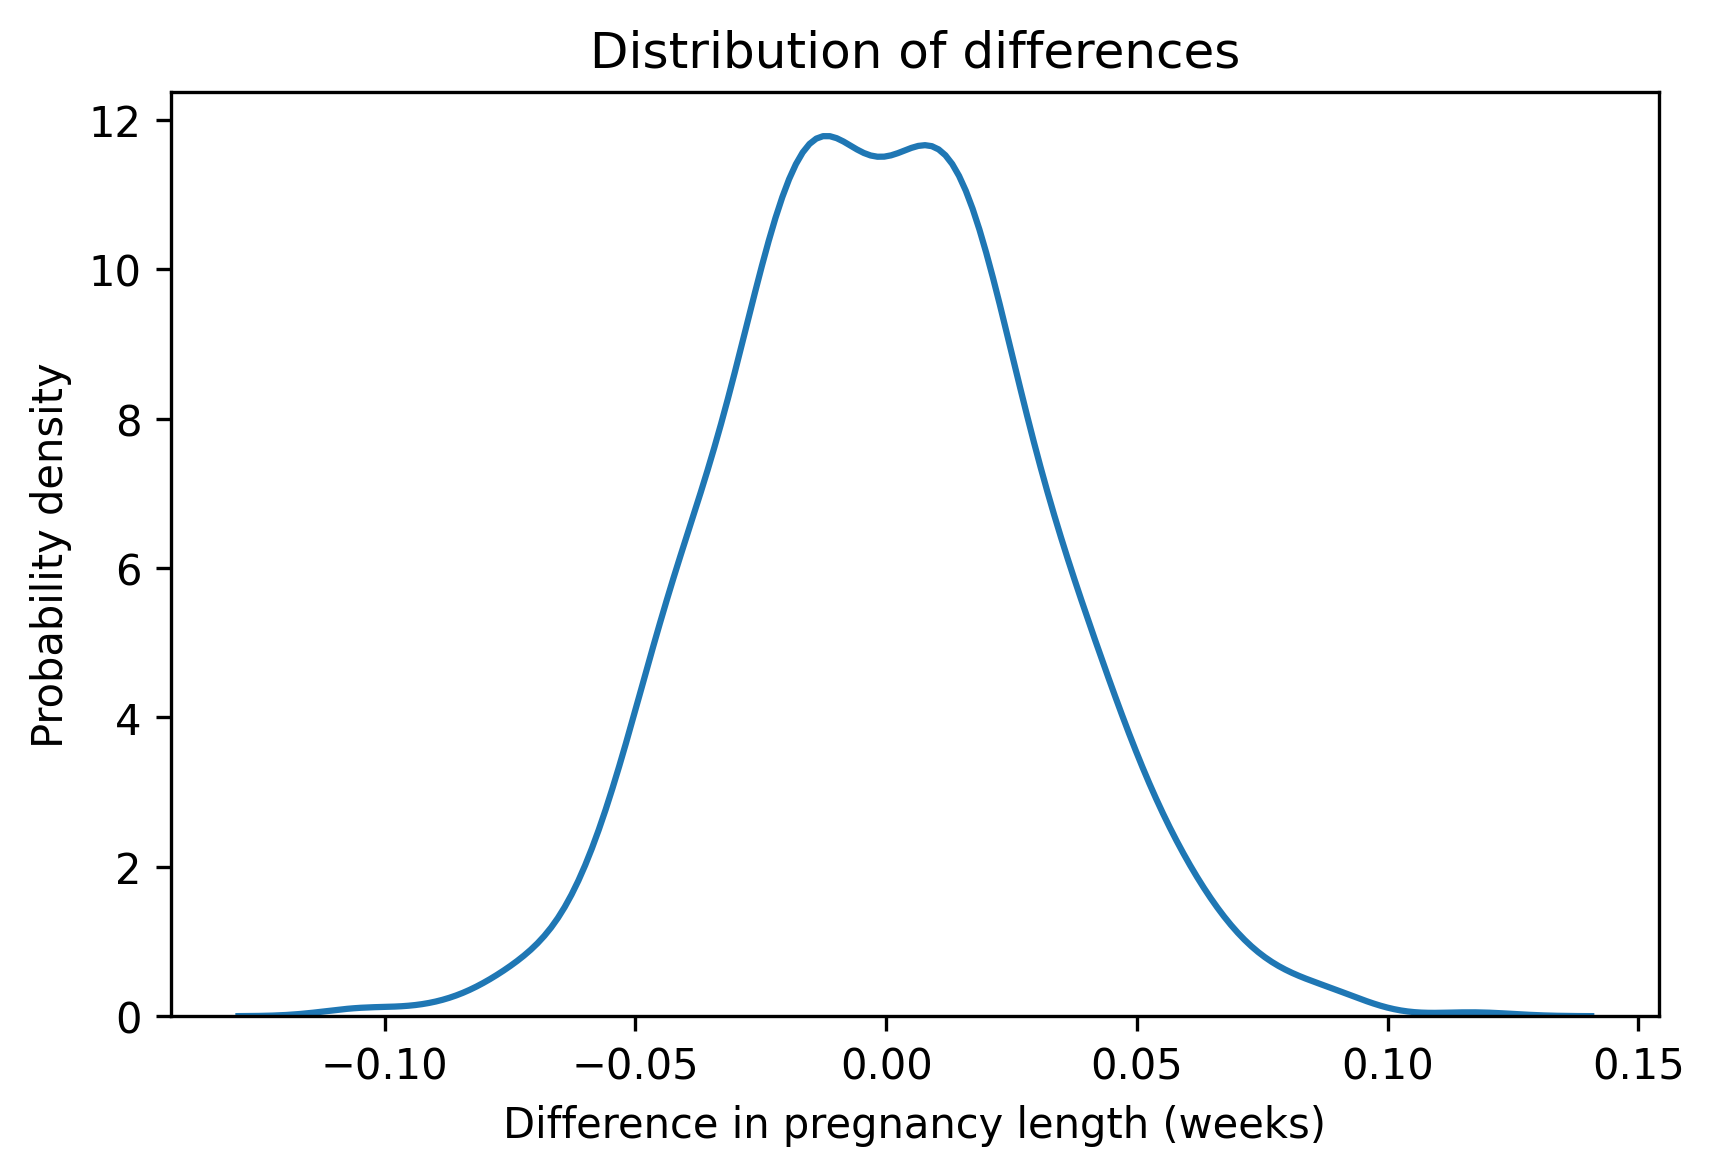
\includegraphics[width=4in]{chapters/13_hypothesis_files/13_hypothesis_65_0.png}
\end{center}

The center of this distribution is near zero, which makes sense if the
distribution in both group is the same. Just by chance, we sometimes see
differences as big as 0.1 weeks, but in 1000 simulations, we never see a
difference as big as the observed difference in the data, which is
almost 0.2 weeks.

Based on this result, we can pretty much rule out the possibility that
the difference we saw is due to random sampling. But we should remember
that there are other possible sources of error. For one, pregnancy
lengths in the NSFG are self-reported. When the respondents are
interviewed, their recollection of first babies might be less accurate
than their recollection of more recent babies. Or the estimation of
pregnancy length might be less accurate with less experienced mothers.

A correspondent of mine, who knows more than me about giving birth,
suggested yet another possibility. If a first baby is born by
\href{https://en.wikipedia.org/wiki/Caesarean_section}{Caesarean
section}, it is more likely that subsequent deliveries will be
scheduled, and less likely that they will go much past 39 weeks. So that
could bring the average down for non-first babies.

In summary, the results in this section suggest that the observed
difference is unlikely to be due to chance, but there are other possible
explanations.

\hypertarget{the-hypothesis-testing-framework}{%
\section{The Hypothesis Testing
Framework}\label{the-hypothesis-testing-framework}}

The examples we've done so far fit into the framework shown in this
diagram:

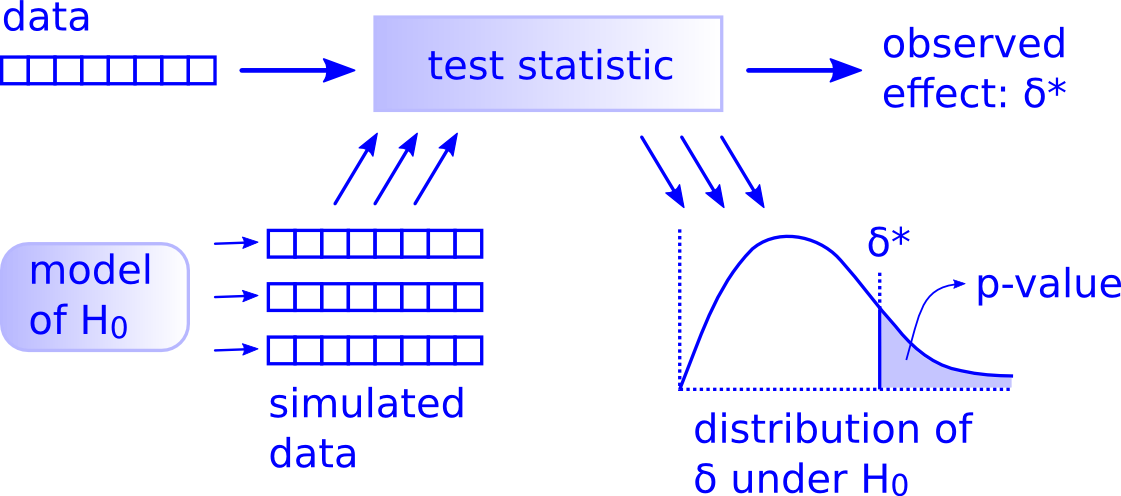
\includegraphics{chapters/figs/hypothesis_testing.png}

Using data from an experiment, we compute the observed \textbf{test
statistic}, denoted \(\delta^*\) in the diagram, which quantifies the
size of the observed effect. In the peanut allergy example, the test
statistic is relative risk. In the pregnancy length example, it is the
difference in the means.

Then we build a model of a world where the effect does not exist. This
model is called the \textbf{null hypothesis} and denoted \(H_0\). In the
peanut allergy example, the model assumes that the risk is the same in
both groups. In the pregnancy example, it assumes that the lengths are
drawn from the same normal distribution.

Next we use the model to simulate the experiment many times. Each
simulation generates a dataset which we use to compute a test statistic,
\(\delta\). Finally, we collect the test statistics from the simulations
and compute a p-value, which is the probability under the null
hypothesis of seeing a test statistic as big as the observed effect,
\(\delta*\).

If the p-value is small, we can usually rule out the possibility that
the observed effect is due to random variation. But often there are
other explanations we can't rule out, including measurement error and
unrepresentative sampling.

I emphasize the role of the model in this framework because for a given
experiment there might be several possible models, each including some
elements of the real world and ignoring others. For example, we used a
normal distribution to model variation in pregnancy length. If we don't
want to make this assumption, an alternative is to simulate the null
hypothesis by shuffling the pregnancy lengths.

The following function takes two sequences representing the pregnancy
lengths for the two groups. It appends them into a single sequence,
shuffles it, and then splits it again into groups with the same size as
the originals. The return value is the difference in means between the
groups.

\begin{lstlisting}[]
def simulate_two_groups(data1, data2):
    n, m = len(data1), len(data2)
    data = np.append(data1, data2)
    np.random.shuffle(data)
    group1 = data[:n]
    group2 = data[n:]
    return group1.mean() - group2.mean()
\end{lstlisting}

If we call this function once, we get a random difference in means from
a simulated world where the distribution of pregnancy lengths is the
same in both groups.

\begin{lstlisting}[]
simulate_two_groups(length_first, length_other)
(@\dashfill@)
@@@-0.03111395525888838@@@
\end{lstlisting}

\textbf{Exercise:} Using this function to run 1000 simulations of the
null hypothesis and save the results as \passthrough{\lstinline!diff2!}.
Make a KDE plot to compare the distribution of
\passthrough{\lstinline!diff2!} to the results from the normal model,
\passthrough{\lstinline!diff!}.

Compute the probability of seeing a difference as big as
\passthrough{\lstinline!diff\_actual!}. Is this p-value consistent with
the results we got with the normal model?

\textbf{Exercise:} Are first babies more likely to be \emph{light}? To
find out, we can use the birth weight data from the NSFG. The variables
we need use special codes to represent missing data, so let's replace
them with \passthrough{\lstinline!NaN!}.

\begin{lstlisting}[]
nsfg['BIRTHWGT_LB1'].replace([0, 98, 99], np.nan, inplace=True)
nsfg['BIRTHWGT_OZ1'].replace([0, 98, 99], np.nan, inplace=True)
\end{lstlisting}

And combine pounds and ounces into a single variable.

\begin{lstlisting}[]
birthwgt = nsfg['BIRTHWGT_LB1'] + nsfg['BIRTHWGT_OZ1'] / 16
\end{lstlisting}

We can use \passthrough{\lstinline!first!} and
\passthrough{\lstinline!other!} to select birth weights for first babies
and others, dropping the \passthrough{\lstinline!NaN!} values.

\begin{lstlisting}[]
birthwgt_first = birthwgt[first].dropna()
birthwgt_other = birthwgt[other].dropna()
\end{lstlisting}

In this dataset, it looks like first babies are a little lighter, on
average.

\begin{lstlisting}[]
print(birthwgt_first.mean(), birthwgt_other.mean())
(@\dashfill@)
@@@7.3370276162790695 7.507115749525616@@@
\end{lstlisting}

But as usual, we should wonder whether we are being fooled by
randomness. To find out, compute the actual difference between the
means. Then use \passthrough{\lstinline!simulate\_two\_groups!} to
simulate a world where birth weights for both groups are drawn from the
same distribution. Under the null hypothesis, how often does the
difference in means exceed the actual difference in the dataset? What
conclusion can you draw from this result?

\hypertarget{testing-correlation}{%
\section{Testing Correlation}\label{testing-correlation}}

The method we used in the previous section is called a
\textbf{permutation test} because we permuted the pregnancy lengths
before dividing them into groups (``permute'' is another word for
shuffle). As another example, in this section we'll use a permutation
tests to check whether an observed correlation might be due to chance.

As an example, let's look again at the correlations we computed in
Chapter 9, using data from the Behavioral Risk Factor Surveillance
System (BRFSS). The following cell reads the data.

\begin{lstlisting}[]
import pandas as pd

brfss = pd.read_hdf('brfss.hdf', 'brfss')
brfss.shape
(@\dashfill@)
@@@(418268, 9)@@@
\end{lstlisting}

The correlations we computed were between height, weight and age.

\begin{lstlisting}[]
columns = ['HTM4', 'WTKG3', 'AGE']
subset = brfss[columns]
corr_actual = subset.corr()
corr_actual
(@\dashfill@)
@@@/home/downey/miniconda3/envs/ElementsOfDataScience/lib/python3.8/site-packages/IPython/core/formatters.py:342: FutureWarning: In future versions `DataFrame.to_latex` is expected to utilise the base implementation of `Styler.to_latex` for formatting and rendering. The arguments signature may therefore change. It is recommended instead to use `DataFrame.style.to_latex` which also contains additional functionality.
  return method()@@@
\end{lstlisting}

\begin{tabular}{lrrr}
\midrule
{} &      HTM4 &     WTKG3 &       AGE \\
\midrule
HTM4  &  1.000000 &  0.477151 & -0.135980 \\
WTKG3 &  0.477151 &  1.000000 & -0.064951 \\
AGE   & -0.135980 & -0.064951 &  1.000000 \\
\midrule
\end{tabular}

The correlation between height and weight is about 0.48, which is
moderately strong; if you know someone's height, you can make a better
guess about their weight. The other correlations are weaker; for
example, knowing someone's age would not substantially improve your
guesses about their height or weight.

Because these correlations are so small, we might wonder whether they
are due to chance. To answer this question, we can use permutation to
simulate a world where there is actually no correlation between two
variables.

But first we have to take a detour to figure out how to shuffle a Pandas
\passthrough{\lstinline!Series!}. As an example, I'll extract the height
data.

\begin{lstlisting}[]
series = brfss['HTM4']
series.head()
\end{lstlisting}

\begin{tabular}{lr}
\midrule
{} &   HTM4 \\
\midrule
0 &  157.0 \\
1 &  163.0 \\
2 &  165.0 \\
3 &  165.0 \\
4 &  152.0 \\
\midrule
\end{tabular}

The idiomatic way to shuffle a \passthrough{\lstinline!Series!} is to
use \passthrough{\lstinline!sample!} with the argument
\passthrough{\lstinline!frac=1!}, which means that the fraction of the
elements we want is \passthrough{\lstinline!1!}, that is, all of them
(see
\url{https://stackoverflow.com/questions/29576430/shuffle-dataframe-rows}).
By default, \passthrough{\lstinline!sample!} chooses elements without
replacement, so the result contains all of the elements in a random
order.

\begin{lstlisting}[]
shuffled = series.sample(frac=1)
shuffled.head()
(@\dashfill@)
@@@/home/downey/miniconda3/envs/ElementsOfDataScience/lib/python3.8/site-packages/IPython/core/formatters.py:342: FutureWarning: In future versions `DataFrame.to_latex` is expected to utilise the base implementation of `Styler.to_latex` for formatting and rendering. The arguments signature may therefore change. It is recommended instead to use `DataFrame.style.to_latex` which also contains additional functionality.
  return method()@@@
\end{lstlisting}

\begin{tabular}{lr}
\midrule
{} &   HTM4 \\
\midrule
205593 &  170.0 \\
292620 &  175.0 \\
44585  &  185.0 \\
13394  &  165.0 \\
67403  &  173.0 \\
\midrule
\end{tabular}

If we check the first few elements, it seems like a random sample, so
that's good. But let's see what happens if we use the shuffled
\passthrough{\lstinline!Series!} to compute a correlation.

\begin{lstlisting}[]
corr = shuffled.corr(brfss['WTKG3'])
corr
(@\dashfill@)
@@@0.4771514628388126@@@
\end{lstlisting}

That result looks familiar: it is the correlation of the unshuffled
columns. The problem is that when we shuffle a
\passthrough{\lstinline!Series!}, the index gets shuffled along with it.
When we compute a correlation, Pandas uses the index to line up the
elements from the first \passthrough{\lstinline!Series!} with the
elements of the second \passthrough{\lstinline!Series!}. For many
operations, that's the behavior we want, but in this case it defeats the
purpose of shuffling!

The solution is to use \passthrough{\lstinline!reset\_index!}, which
gives the \passthrough{\lstinline!Series!} a new index, with the
argument \passthrough{\lstinline!drop=True!}, which drops the old one.
So we have to shuffle \passthrough{\lstinline!series!} like this.

\begin{lstlisting}[]
shuffled = series.sample(frac=1).reset_index(drop=True)
\end{lstlisting}

Now we can compute a correlation with the shuffled
\passthrough{\lstinline!Series!}.

\begin{lstlisting}[]
corr = shuffled.corr(brfss['WTKG3'])
corr
(@\dashfill@)
@@@0.003117718945752241@@@
\end{lstlisting}

The result is small, as we expect it to be when the elements are aligned
at random.

Rather than repeat this awful idiom, let's put it in a function and
never speak of it again.

\begin{lstlisting}[]
def shuffle(series):
    return series.sample(frac=1).reset_index(drop=True)
\end{lstlisting}

The following function takes a \passthrough{\lstinline!DataFrame!} and
two column names, makes a shuffled copy of one column, and computes its
correlation with the other.

\begin{lstlisting}[]
def simulate_correlation(df, var1, var2):
    corr = shuffle(df[var1]).corr(df[var2])
    return corr
\end{lstlisting}

We only have to shuffle one of the columns; it doesn't get any more
random if we shuffle both. Now we can use this function to generate a
sample of correlations with shuffled columns.

\begin{lstlisting}[]
t = [simulate_correlation(brfss, 'HTM4', 'WTKG3')
     for i in range(200)]
\end{lstlisting}

Here's the distribution of the correlations.

\begin{lstlisting}[]
sns.kdeplot(t)

plt.xlabel('Correlation')
plt.ylabel('Probability density')
plt.title('Correlation from simulations with permutation');
\end{lstlisting}

\begin{center}
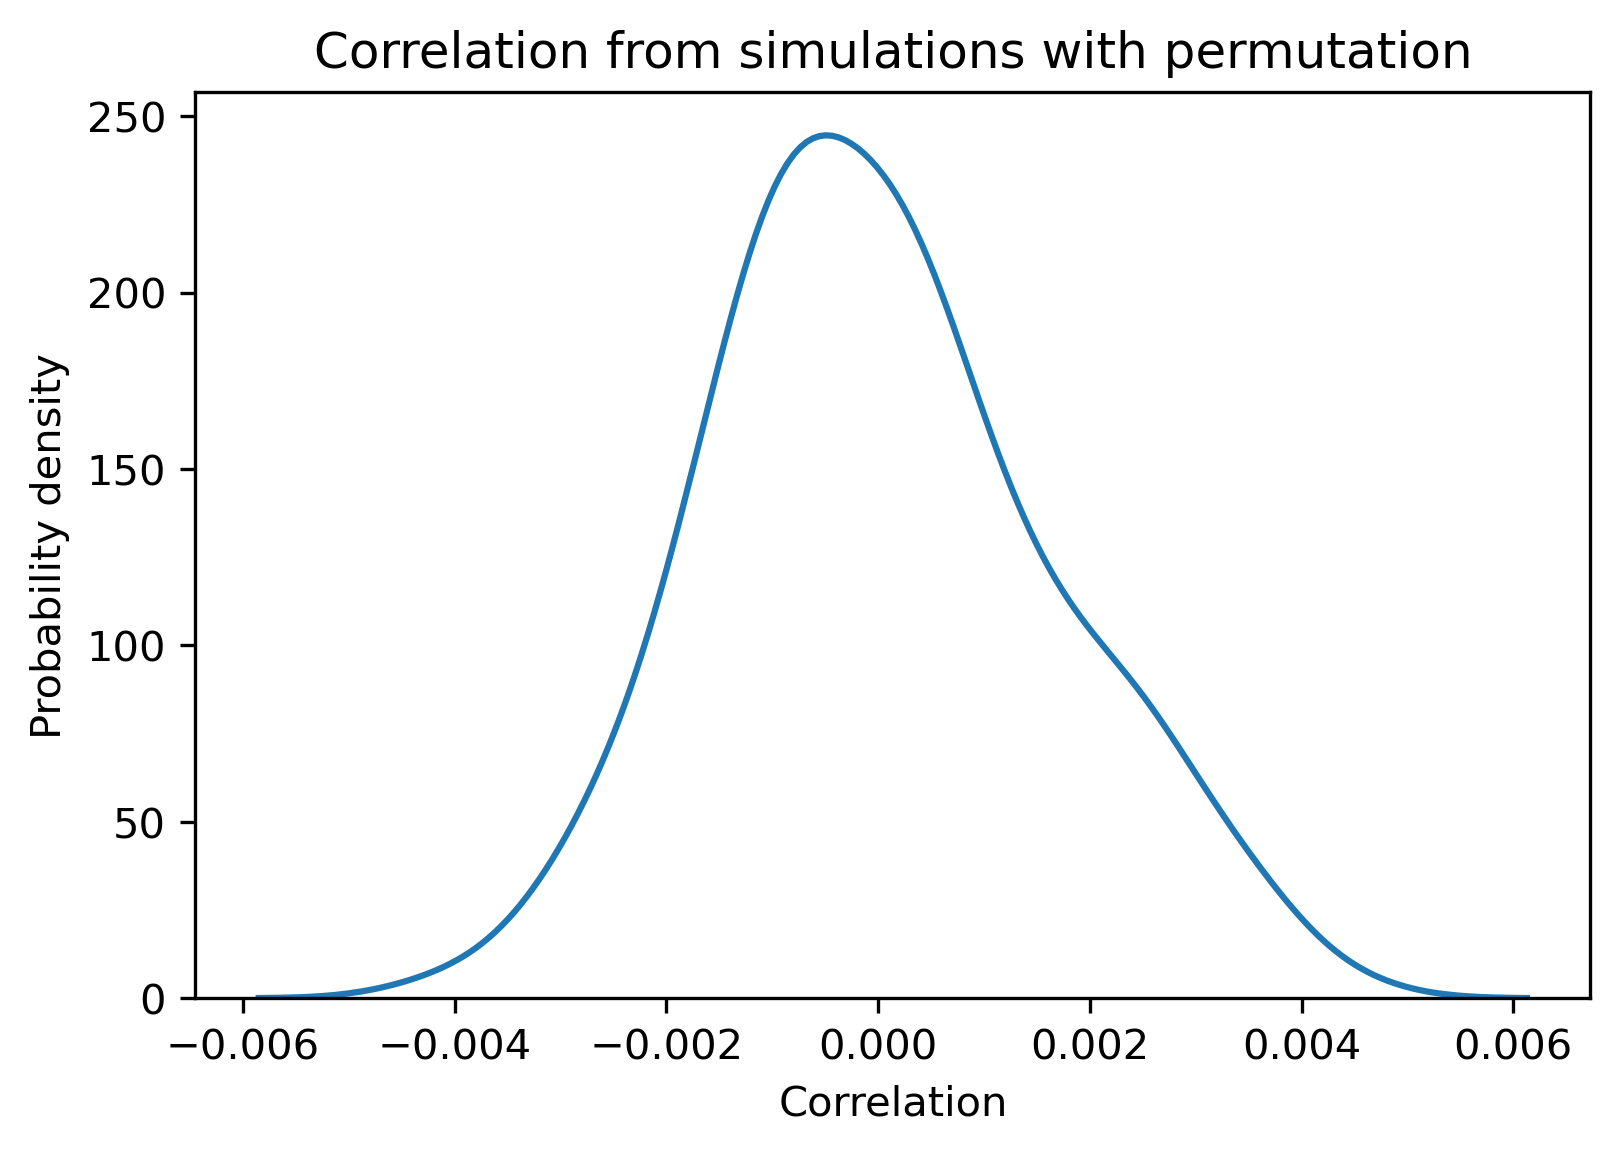
\includegraphics[width=4in]{chapters/13_hypothesis_files/13_hypothesis_107_0.png}
\end{center}

The center of the distribution is near 0, and the largest values
(positive or negative) are around 0.005. If we compute the same
distribution with different columns, the results are pretty much the
same. With samples this big, the correlation between shuffled columns is
generally small.

How do these values compare to the observed correlations?

\begin{itemize}
\item
  The correlation of height and weight is about 0.48, so it's extremely
  unlikely we would see a correlation as big as that by chance.
\item
  The correlation of height and age is smaller, around -0.14, but even
  that value would be unlikely by chance.
\item
  And the correlation of weight and age is even smaller, about -0.06,
  but that's still 10 times bigger than the biggest correlation in the
  simulations.
\end{itemize}

We can conclude that these correlations are probably not due to chance.
And that's useful in the sense that it rules out one possible
explanation. But this example also demonstrates a limitation of this
kind of hypothesis testing. With large sample sizes, variability due to
randomness tends to be small, so it seldom explains the effects we see
in real data.

And hypothesis testing can be a distraction from more important
questions. In Chapter 9, we saw that the relationship between weight and
age is nonlinear. But the coefficient of correlation only measures
linear relationships, so it does not capture the real strength of the
relationship. So testing a correlation might not be the more useful
thing to do in the first place. We can do better by testing a regression
model.

\hypertarget{testing-regression-models}{%
\section{Testing Regression Models}\label{testing-regression-models}}

In the previous sections we used permutation to simulate a world where
there is no correlation between two variables. In this section we'll
apply the same method to regression models.

As an example, we'll use NSFG data to explore the relationship between a
mother's age and her baby's birth weight.

In previous sections we computed birth weight and a Boolean variable
that identifies first babies. Now we'll store them as columns in
\passthrough{\lstinline!nsfg!}, so we can use them with StatsModels.

\begin{lstlisting}[]
nsfg['BIRTHWGT'] = birthwgt
nsfg['FIRST'] = first
\end{lstlisting}

We can select the subset of the rows that represent live, full-term
births, and make a copy so we can modify the subset without affecting
the original.

\begin{lstlisting}[]
subset = nsfg[live & fullterm].copy()
n = len(subset)
n
(@\dashfill@)
@@@5839@@@
\end{lstlisting}

To visualize the relationship between mother's age and birth weight,
we'll use a box plot with mother's age grouped into 3-year bins. We can
use \passthrough{\lstinline!np.arange!} to make the bin boundaries, and
\passthrough{\lstinline!pd.cut!} to put the values from
\passthrough{\lstinline!AGECON!} into bins.

\begin{lstlisting}[]
bins = np.arange(15, 40, 3)
labels = (bins + 1)[:-1]

subset['AGEGRP'] = pd.cut(subset['AGECON'], 
                          bins, labels=labels)
\end{lstlisting}

The label for each bin is the midpoint of the range; I used a slice to
remove the last label because the number of bins is one less than the
number of bin boundaries.

Here's the box plot.

\begin{lstlisting}[]
sns.boxplot(x='AGEGRP', y='BIRTHWGT', data=subset, 
            whis=None, color='plum')

plt.xlabel("Mother's age (years)")
plt.ylabel('Birthweight (pounds)');
\end{lstlisting}

\begin{center}
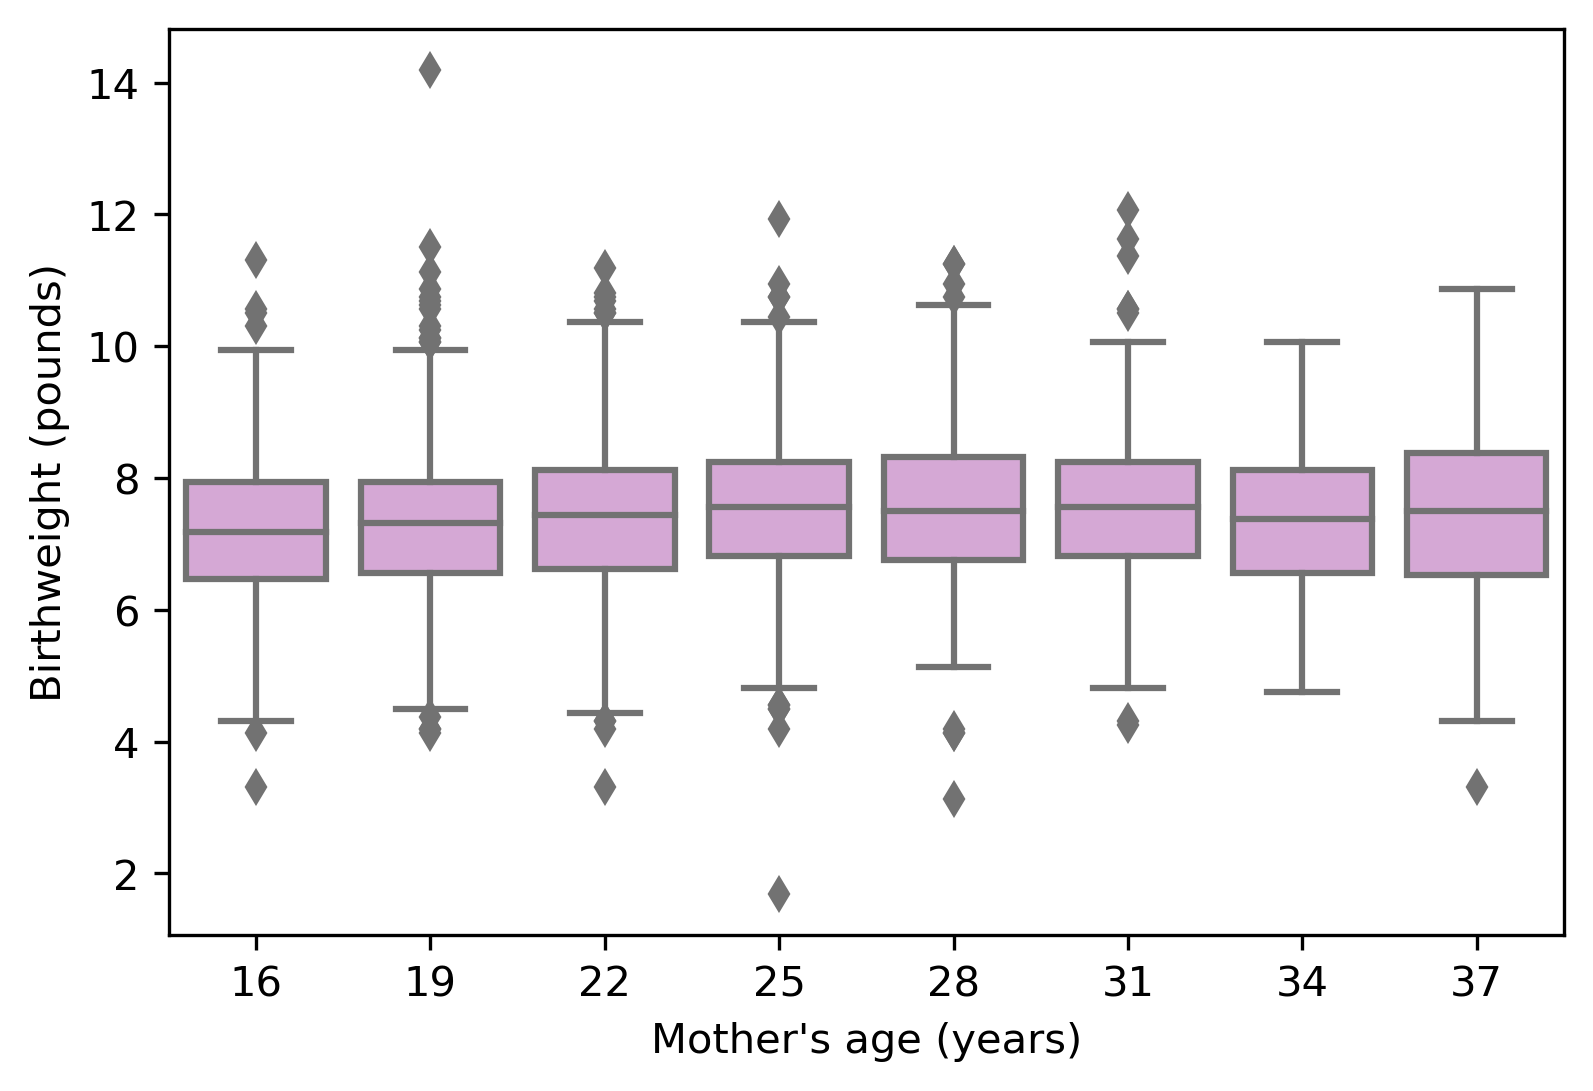
\includegraphics[width=4in]{chapters/13_hypothesis_files/13_hypothesis_117_0.png}
\end{center}

It looks like the average birth weight is highest if the mother is 25-31
years old, and lower if she is younger or older. So the relationship
might be nonlinear. Nevertheless, let's start with a linear model and
work our way up. Here's a simple regression of birth weight as a
function of the mother's age at conception.

\begin{lstlisting}[]
import statsmodels.formula.api as smf

results = smf.ols('BIRTHWGT ~ AGECON', data=subset).fit()
results.params
(@\dashfill@)
@@@/home/downey/miniconda3/envs/ElementsOfDataScience/lib/python3.8/site-packages/IPython/core/formatters.py:342: FutureWarning: In future versions `DataFrame.to_latex` is expected to utilise the base implementation of `Styler.to_latex` for formatting and rendering. The arguments signature may therefore change. It is recommended instead to use `DataFrame.style.to_latex` which also contains additional functionality.
  return method()@@@
\end{lstlisting}

\begin{tabular}{lr}
\midrule
{} &         0 \\
\midrule
Intercept &  7.025486 \\
AGECON    &  0.016407 \\
\midrule
\end{tabular}

The slope of the regression line is 0.016 pounds per year, which means
that if one mother is a year older than another, we expect her baby to
be about 0.016 pounds heavier, which is about a quarter of an ounce.

This parameter is small, so we might wonder whether the apparent effect
is due to chance. To answer that question, we will use permutation to
simulate a world where there is no relationship between mother's age and
birth weight.

As a test statistic, we'll use the coefficient of determination, denoted
\(R^2\), which quantifies the predictive power of the model (see
\url{https://en.wikipedia.org/wiki/Coefficient_of_determination}). The
regression results include \(R^2\) in a variable called
\passthrough{\lstinline!rsquared!}.

\begin{lstlisting}[]
results.rsquared
(@\dashfill@)
@@@0.007578923866134457@@@
\end{lstlisting}

The value of \(R^2\) for this model is very small, which means that our
guesses about a baby's weight are barely improved if we know the
mother's age (and use a linear model). So it seems possible that the
apparent relationship between these variables is due to chance. We can
test this possibility by using permutation to simulate a world where
there is no such relationship.

The following function takes a \passthrough{\lstinline!DataFrame!},
shuffles the \passthrough{\lstinline!AGECON!} column, computes a linear
regression model, and returns \(R^2\).

\begin{lstlisting}[]
def simulate_rsquared(df):
    df['SHUFFLED'] = shuffle(df['AGECON'])
    formula = 'BIRTHWGT ~ SHUFFLED'
    results = smf.ols(formula, data=df).fit()
    return results.rsquared
\end{lstlisting}

If we call it many times, we get a sample from the distribution of
\(R^2\) under the null hypothesis.

\begin{lstlisting}[]
rsquared_null = [simulate_rsquared(subset)
                 for i in range(200)]
\end{lstlisting}

After 200 attempts, the largest value of \(R^2\) is about 0.003, which
is smaller than the observed value of \(R^2\), about 0.008. We conclude
that the observed effect is bigger than we would expect to see by
chance.

\begin{lstlisting}[]
print(np.max(rsquared_null), results.rsquared)
(@\dashfill@)
@@@0.00336666951682707 0.007578923866134457@@@
\end{lstlisting}

\textbf{Exercise:} The box plot suggests that the relationship between
mother's age and birth weight is nonlinear, so let's try a nonlinear
model. I'll add a column to the \passthrough{\lstinline!DataFrame!} with
the square of mother's age.

\begin{lstlisting}[]
subset['AGECON2'] = subset['AGECON']**2
\end{lstlisting}

And run the model again with both the linear and quadratic terms.

\begin{lstlisting}[]
formula = 'BIRTHWGT ~ AGECON + AGECON2'
results2 = smf.ols(formula, data=subset).fit()
results2.params
(@\dashfill@)
@@@/home/downey/miniconda3/envs/ElementsOfDataScience/lib/python3.8/site-packages/IPython/core/formatters.py:342: FutureWarning: In future versions `DataFrame.to_latex` is expected to utilise the base implementation of `Styler.to_latex` for formatting and rendering. The arguments signature may therefore change. It is recommended instead to use `DataFrame.style.to_latex` which also contains additional functionality.
  return method()@@@
\end{lstlisting}

\begin{tabular}{lr}
\midrule
{} &         0 \\
\midrule
Intercept &  5.894125 \\
AGECON    &  0.109487 \\
AGECON2   & -0.001810 \\
\midrule
\end{tabular}

The parameter of \passthrough{\lstinline!AGECON2!} is quite small, so we
might wonder whether it actually improves the model, or might be the
product of randomness. One way to answer this question is to look at the
improvement in \(R^2\).

\begin{lstlisting}[]
results2.rsquared
(@\dashfill@)
@@@0.011861010196576371@@@
\end{lstlisting}

The value of \(R^2\) is about 0.012, compared to 0.008 with the linear
model. By this criterion, the quadratic model is a better, but when we
add variables to a model, we might get some improvement just by chance.
To see how much, write a function called
\passthrough{\lstinline!simulate\_rsquared2!} that takes a
\passthrough{\lstinline!DataFrame!} as a parameter, shuffles
\passthrough{\lstinline!AGECON2!}, runs a regression model with
\passthrough{\lstinline!AGECON!} and the shuffled values, and returns
\(R^2\). Run your function 200 times and count how often \(R^2\) from
the model exceeds the observed value from the dataset. What conclusion
can you draw?

\hypertarget{controlling-for-age}{%
\section{Controlling for Age}\label{controlling-for-age}}

In a previous exercise, you computed the difference in birth weight
between first babies and others, which is about 0.17 pounds, and you
checked whether we are likely to see a difference as big as that by
chance. If things went according to plan, you found that it is very
unlikely.

But that doesn't necessarily mean that there is anything special about
first babies that makes them lighter than others. Rather, knowing a
baby's birth order might provide information about some other factor
that is related to birth weight. The mother's age could be that factor.

First babies are likely to have younger mothers than other babies, and
younger mothers tend to have lighter babies. The difference we see in
first babies might be explained by their mothers' ages. So let's see
what happens if we control for age. Here's a simple regression of birth
weight as a function of the Boolean variable
\passthrough{\lstinline!FIRST!}.

\begin{lstlisting}[]
formula = 'BIRTHWGT ~ FIRST'
results = smf.ols(formula, data=subset).fit()
results.params
(@\dashfill@)
@@@/home/downey/miniconda3/envs/ElementsOfDataScience/lib/python3.8/site-packages/IPython/core/formatters.py:342: FutureWarning: In future versions `DataFrame.to_latex` is expected to utilise the base implementation of `Styler.to_latex` for formatting and rendering. The arguments signature may therefore change. It is recommended instead to use `DataFrame.style.to_latex` which also contains additional functionality.
  return method()@@@
\end{lstlisting}

\begin{tabular}{lr}
\midrule
{} &         0 \\
\midrule
Intercept     &  7.507116 \\
FIRST[T.True] & -0.170088 \\
\midrule
\end{tabular}

The parameter associated with \passthrough{\lstinline!FIRST!} is -0.17
pounds, which is the same as the difference in means we computed. But
now we can add \passthrough{\lstinline!AGECON!} as a control variable.

\begin{lstlisting}[]
formula = 'BIRTHWGT ~ FIRST + AGECON'
results = smf.ols(formula, data=subset).fit()
results.params
(@\dashfill@)
@@@/home/downey/miniconda3/envs/ElementsOfDataScience/lib/python3.8/site-packages/IPython/core/formatters.py:342: FutureWarning: In future versions `DataFrame.to_latex` is expected to utilise the base implementation of `Styler.to_latex` for formatting and rendering. The arguments signature may therefore change. It is recommended instead to use `DataFrame.style.to_latex` which also contains additional functionality.
  return method()@@@
\end{lstlisting}

\begin{tabular}{lr}
\midrule
{} &         0 \\
\midrule
Intercept     &  7.163240 \\
FIRST[T.True] & -0.121771 \\
AGECON        &  0.013145 \\
\midrule
\end{tabular}

The age effect accounts for some of the difference between first babies
and others. After controlling for age, the remaining difference is about
0.12 pounds. Since the age effect is nonlinear, we can can control for
age more effectively by adding \passthrough{\lstinline!AGECON2!}.

\begin{lstlisting}[]
formula = 'BIRTHWGT ~ FIRST + AGECON + AGECON2'
results = smf.ols(formula, data=subset).fit()
results.params
(@\dashfill@)
@@@/home/downey/miniconda3/envs/ElementsOfDataScience/lib/python3.8/site-packages/IPython/core/formatters.py:342: FutureWarning: In future versions `DataFrame.to_latex` is expected to utilise the base implementation of `Styler.to_latex` for formatting and rendering. The arguments signature may therefore change. It is recommended instead to use `DataFrame.style.to_latex` which also contains additional functionality.
  return method()@@@
\end{lstlisting}

\begin{tabular}{lr}
\midrule
{} &         0 \\
\midrule
Intercept     &  6.128590 \\
FIRST[T.True] & -0.099338 \\
AGECON        &  0.096781 \\
AGECON2       & -0.001615 \\
\midrule
\end{tabular}

\begin{lstlisting}[]
slope_actual = results.params['FIRST[T.True]']
slope_actual
(@\dashfill@)
@@@-0.09933806121560428@@@
\end{lstlisting}

When we use a quadratic model to control for the age effect, the
remaining difference between first babies and others is smaller again,
about 0.10 pounds.

One of the warning signs of a spurious relationship between two
variables is that the effect gradually disappears as you add control
variables. So we should wonder whether the remaining effect might be due
to chance. To find out, we'll use the following function, which
simulates a world where there is no difference in weight between first
babies and others. It takes a \passthrough{\lstinline!DataFrame!} as a
parameter, shuffles the \passthrough{\lstinline!FIRST!} column, runs the
regression model with \passthrough{\lstinline!AGECON!} and
\passthrough{\lstinline!AGECON2!}, and returns the estimated difference.

\begin{lstlisting}[]
def simulate_slope(df):
    df['SHUFFLED'] = shuffle(df['FIRST'])
    formula = 'BIRTHWGT ~ AGECON + AGECON2 + C(SHUFFLED)'
    results = smf.ols(formula, data=df).fit()
    return results.params['C(SHUFFLED)[T.True]']
\end{lstlisting}

If we run it many times, we get a sample from the distribution of the
test statistic under the null hypothesis.

\begin{lstlisting}[]
slopes_null = [simulate_slope(subset)
               for i in range(200)]
\end{lstlisting}

The range of values is wide enough that it occasionally exceeds the
observed effect size.

\begin{lstlisting}[]
print(min(slopes_null), max(slopes_null))
(@\dashfill@)
@@@-0.10810723399823335 0.12738249958193174@@@
\end{lstlisting}

Our estimate of the p-value is only approximate, but it looks like it's
between 1\% and 2\%.

\begin{lstlisting}[]
p_value = (np.abs(slopes_null) > np.abs(slope_actual)).mean()
p_value
(@\dashfill@)
@@@0.015@@@
\end{lstlisting}

This result indicates that an observed difference of 0.1 pounds is
possible, but not likely, if the actual difference between the groups is
zero.

So how should we interpret a result like this? In the tradition of
statistical hypothesis testing, it is common to use 5\% as the threshold
between results that are considered ``statistically significant'' or not
(see
\url{https://en.wikipedia.org/wiki/Statistical_hypothesis_testing}). By
that standard, the weight difference between first babies and others is
statistically significant.

However, there are several problems with this practice:

\begin{itemize}
\item
  First, the choice of the threshold should depend on the context. For a
  life-and-death decision, we might choose a more stringent threshold.
  For a topic of idle curiosity, like this one, we could be more
  relaxed.
\item
  But it might not be useful to apply a threshold at all. An alternative
  (which is common in practice) is to report the p-value and let it
  speak for itself. It provides no additional value to declare that the
  result is significant or not.
\item
  Finally, the use of the word ``significant'' is dangerously
  misleading, because it implies that the result is important in
  practice. But a small p-value only means that an observed effect would
  be unlikely to happen by chance. It doesn't mean it is important.
\end{itemize}

This last point is particularly problematic with large datasets, because
very small effects can be statistically significant. We saw an example
with the BRFSS dataset, where the correlations we tested were \emph{all}
statistically significant, even the ones that are too small to matter in
practice.

\hypertarget{summary}{%
\section{Summary}\label{summary}}

Let's review the examples in this chapter:

\begin{enumerate}
\def\labelenumi{\arabic{enumi}.}
\item
  We started with data from LEAP, which studied the effect of eating
  peanuts on the development of peanut allergies. The test statistic was
  relative risk, and the null hypothesis was that the treatment was
  ineffective.
\item
  Then we looked at the difference in pregnancy length for first babies
  and others. We used the difference in means as the test statistic, and
  two models of the null hypothesis: one based on a normal model and the
  other based on permutation of the data. As an exercise, you tested the
  difference in weight between first babies and others.
\item
  Next we used permutation to test correlations, using height, weight,
  and age data from the BRFSS. This example shows that with large sample
  sizes, observed effects are often ``statistically significant'', even
  if they are too small to matter in practice.
\item
  We used regression models to explore the maternal age effect on birth
  weight. To see whether the effect might be due to chance, we used
  permutation to model the null hypothesis and \(R^2\) as a test
  statistic.
\item
  Finally, we explored the possibility that the first baby effect is
  actually an indirect maternal age effect. After controlling for the
  mother's age, we tested whether the remaining difference between first
  babies and others might happen by chance. We used permutation to model
  the null hypothesis and the estimated slope as a test statistic.
\end{enumerate}

As a final exercise, below, you can use the same methods to explore the
paternal age effect.

\textbf{Exercise:} A paternal age effect is a relationship between the
age of a father and a variety of outcomes for their children (see
\url{https://en.wikipedia.org/wiki/Paternal_age_effect}). There is some
evidence that young fathers and old fathers tend to have lighter babies
than fathers in the middle. Let's see if that's true for the babies in
the NSFG dataset. The \passthrough{\lstinline!HPAGELB!} column encodes
the father's age. Here are the values, after replacing the codes for
missing data with \passthrough{\lstinline!NaN!}.

\begin{lstlisting}[]
subset['HPAGELB'].replace([98, 99], np.nan, inplace=True)
subset['HPAGELB'].value_counts().sort_index()
(@\dashfill@)
@@@/home/downey/miniconda3/envs/ElementsOfDataScience/lib/python3.8/site-packages/IPython/core/formatters.py:342: FutureWarning: In future versions `DataFrame.to_latex` is expected to utilise the base implementation of `Styler.to_latex` for formatting and rendering. The arguments signature may therefore change. It is recommended instead to use `DataFrame.style.to_latex` which also contains additional functionality.
  return method()@@@
\end{lstlisting}

\begin{tabular}{lr}
\midrule
{} &  HPAGELB \\
\midrule
1.0 &      478 \\
2.0 &     1391 \\
3.0 &     1650 \\
4.0 &     1225 \\
5.0 &      592 \\
6.0 &      411 \\
\midrule
\end{tabular}

And here's what the codes mean:

\begin{longtable}[]{@{}ll@{}}
\midrule()
Code & Age \\
\midrule()
\endhead
1 & Under 20 years \\
2 & 20-24 years \\
3 & 25-29 years \\
4 & 30-34 years \\
5 & 35-39 years \\
6 & 40 years or older \\
\midrule()
\end{longtable}

Let's create a new column that's true for the fathers in the youngest
and oldest groups.

\begin{lstlisting}[]
subset['YO_DAD'] = subset['HPAGELB'].isin([1, 6])
\end{lstlisting}

We can use this column in a regression model to compute the difference
in birth weight for young and old fathers compared to the others.

\begin{lstlisting}[]
formula = 'BIRTHWGT ~ YO_DAD'
results = smf.ols(formula, data=subset).fit()
results.params
(@\dashfill@)
@@@/home/downey/miniconda3/envs/ElementsOfDataScience/lib/python3.8/site-packages/IPython/core/formatters.py:342: FutureWarning: In future versions `DataFrame.to_latex` is expected to utilise the base implementation of `Styler.to_latex` for formatting and rendering. The arguments signature may therefore change. It is recommended instead to use `DataFrame.style.to_latex` which also contains additional functionality.
  return method()@@@
\end{lstlisting}

\begin{tabular}{lr}
\midrule
{} &         0 \\
\midrule
Intercept      &  7.447477 \\
YO\_DAD[T.True] & -0.140045 \\
\midrule
\end{tabular}

The difference is negative, which is consistent with the theory, and
about 0.14 pounds, which is comparable in size to the (apparent) first
baby effect. But there is a strong correlation between father's age and
mother's age. So what seems like a paternal age effect might actually be
an indirect maternal age effect. To find out, let's see what happens if
we control for the mother's age. Run this model again with
\passthrough{\lstinline!AGECON!} and \passthrough{\lstinline!AGECON2!}
as predictors. Does the observed effect of paternal age get smaller?

To see if the remaining effect could be due to randomness, write a
function that shuffles \passthrough{\lstinline!YO\_DAD!}, runs the
regression model, and returns the parameter associated with the shuffled
column. How often does this parameter exceed the observed value? What
conclusion can we draw from the results?

